% Created 2022-06-13 Mon 13:13
% Intended LaTeX compiler: pdflatex
\documentclass[smaller]{beamer}\usepackage{listings}
\usepackage{color}
\usepackage{amsmath}
\usepackage{array}
\usepackage[T1]{fontenc}
\usepackage{natbib}
\lstset{
keywordstyle=\color{blue},
commentstyle=\color{red},stringstyle=\color[rgb]{0,.5,0},
literate={~}{$\sim$}{1},
basicstyle=\ttfamily\small,
columns=fullflexible,
breaklines=true,
breakatwhitespace=false,
numbers=left,
numberstyle=\ttfamily\tiny\color{gray},
stepnumber=1,
numbersep=10pt,
backgroundcolor=\color{white},
tabsize=4,
keepspaces=true,
showspaces=false,
showstringspaces=false,
xleftmargin=.23in,
frame=single,
basewidth={0.5em,0.4em},
}
\institute{PhD Student, Section of Biostatistics \\ University of Copenhagen}
\usepackage{natbib, dsfont, pgfpages, tikz,amssymb, amsmath,xcolor}
\bibliographystyle{abbrvnat}
% New operators and commands
\newcommand{\Z}{\mathbb{Z}}
\newcommand{\Q}{\mathbb{Q}}
\newcommand{\R}{\mathbb{R}}
\newcommand{\N}{\mathbb{N}}
\newcommand{\C}{\mathbb{C}}
\renewcommand{\S}{\mathbb{S}}
\newcommand{\blank}{\makebox[1ex]{\textbf{$\cdot$}}}
\newcommand\independent{\protect\mathpalette{\protect\independenT}{\perp}}
\def\independenT#1#2{\mathrel{\rlap{$#1#2$}\mkern2mu{#1#2}}}
\renewcommand{\phi}{\varphi}
\renewcommand{\epsilon}{\varepsilon}
\newcommand*\diff{\mathop{}\!\mathrm{d}}
\newcommand{\weakly}{\rightsquigarrow}
\newcommand\smallO{
  \mathchoice
    {{\scriptstyle\mathcal{O}}}% \displaystyle
    {{\scriptstyle\mathcal{O}}}% \textstyle
    {{\scriptscriptstyle\mathcal{O}}}% \scriptstyle
    {\scalebox{.6}{$\scriptscriptstyle\mathcal{O}$}}%\scriptscriptstyle
}
\newcommand{\midd}{\; \middle|\;}
\newcommand{\1}{\mathds{1}}
\usepackage{ifthen} %% Empirical process with default argument
% \newcommand{\G}[1][]{%
%    \ifthenelse{ \equal{#1}{} }
%       {\ensuremath{\mathbb{G}_n}}
%       {\ensuremath{\mathbb{G}_{#1}}}
% }
% New version:
\newcommand{\G}[2][n]{
{\ensuremath{\mathbb{G}_{#1}}{\left[#2\right]}}
}
\DeclareMathOperator*{\argmin}{\arg\!\min}

% New operators for consistent notation
\newcommand{\V}{\mathrm{Var}} % variance
\newcommand{\measure}[1]{\mathrm{{#1}}} % measure
% \newcommand{\measure}[1]{\textnormal{\textbf{{#1}}}} % measure
\newcommand{\m}[1]{\measure{#1}} % measure shortcut
\newcommand{\eqd}{\stackrel{d}{=}} % equality in distribution
\newcommand{\arrow}[1]{\xrightarrow{\; {#1} \;}}
\newcommand{\arrowP}{\xrightarrow{\; \m{P} \;}} % convergence in probability
\newcommand{\leb}{\lambda} % the Lebesgue measure
\newcommand{\T}{\top} % transpose
\newcommand{\KL}{\ensuremath{D_{\mathrm{KL}}}}

\usepackage{xargs}
% Make it easy to change counterfactual notation:
\newcommandx{\cf}[4][3={}, 4={}]{
  % \ifthenelse{ \equal{#4}{} }
  % {{#1^{#2}}(#3)}
  {\ifthenelse{ \equal{#3}{} }
    {{#1^{#2}}_{#4}}
    {{#1^{#2}}_{#4}(#3)}}
}

% Easily change notation:
\DeclareMathOperator{\TT}{\Psi} % target parameter
\newcommand{\lp}{\mathcal{L}_{\P}^2} % shortcut for lp2 space
\newcommand{\empmeas}{\hat{\mathbb{P}}_n} % empirical measure
\DeclareMathOperator{\E}{\mathbb{E}} % expectation
\renewcommand{\P}{\m{P}} % probability
\newcommand{\ic}{\mathrm{IF}} % influence curve
\setbeamertemplate{footline}[frame number]
\beamertemplatenavigationsymbolsempty
\usepackage{appendixnumberbeamer}
\setbeamercolor{gray}{bg=white!90!black}
\setbeamertemplate{itemize items}{$\circ$}

\renewcommand*\familydefault{\sfdefault}
\itemsep2pt
\usepackage[utf8]{inputenc}
\usepackage[T1]{fontenc}
\usepackage{graphicx}
\usepackage{longtable}
\usepackage{wrapfig}
\usepackage{rotating}
\usepackage[normalem]{ulem}
\usepackage{amsmath}
\usepackage{amssymb}
\usepackage{capt-of}
\usepackage{hyperref}
\usetheme{default}
\author{Anders Munch}
\date{\today}
\title{The negative log-likelihood loss and cross-validation with censored data}
\begin{document}

\maketitle
\begin{frame}{Outline}
\tableofcontents
\end{frame}

\section{Problem setting: Model and hyperparamter selection for survival model}
\label{sec:orgfbb9f88}
\begin{frame}[label={sec:orgf50e91a}]{Selecting a model from a collection of candidate models}
\small Let \(\mathcal{P}\) denote a collection of probability measures on the sample space
\(\mathcal{O}\). Let \(\mathcal{V}\) denote a parameter space and \(L\colon\mathcal{V} \times \mathcal{O}
\rightarrow \R_+\) a loss function. Consider

\begin{equation*}
  \nu(P) := \argmin_{\tilde{\nu}\in\mathcal{V}} P[L(\tilde{\nu}, \blank)],
  \quad \text{where} \quad
  P[f] := \int_{\mathcal{O}}f(o) P(\diff o). 
\end{equation*}
We approximate $P$ with the empirical measure $\empmeas$, as
$\empmeas[L(\tilde{\nu}, \blank)] \approx P[L(\tilde{\nu}, \blank)]$.
% $\nu(\empmeas)\approx\nu(P)$.

\begin{exampleblock}{Maximum likelihood estimator (MLE)}
For \(\mathcal{V}\) a collection of densities and \(L(\nu,O) := -\log(\nu(O))\), \(\nu(\empmeas)\) is
the MLE.
\end{exampleblock}

\begin{exampleblock}{Hyper-parameter selection}
For estimation in high-dimensional settings we often introduce a regularization parameter \(\nu\)
(e.g., LASSO, kernel smoothing). Each choice of \(\nu\) gives us an estimator, say \(\hat f_{\nu}\), and
we select the optimal choice of \(\nu\) using cross-validation,
\begin{equation*}
  \argmin_{\nu\in\mathcal{V}} \empmeas[L(\hat{f}_{\nu}, \blank)],
  \quad \text{where} \quad
  \empmeas \independent \hat{f}_{\nu}.
\end{equation*}
Also useful for combining models \citep{breiman1996stacked,van2007super}.
\end{exampleblock}
\end{frame}

\begin{frame}[label={sec:org31fa036}]{Survival data}
\small

\begin{description}
\item[{\(O = (\tilde T, \Delta, X) \sim P \in \mathcal{P}\)}] Oberved data with \(\mathcal{O} = \R_+
  \times \{0,1\} \times \R^p\).
\item[{\((T, X) \sim Q \in \mathcal{Q}\)}] The distribution \(Q\) (or a feature of it) is of interest.
\end{description}

\vfill

Assuming coarsening at random \citep{gill1997coarsening} we can write
\begin{equation*}
  \mathcal{P} = \{P_{Q, G} : Q \in \mathcal{Q}, G \in \mathcal{G}\},
\end{equation*}
where $\mathcal{G}$ denotes a collection of conditional distributions for the censoring mechanism.
Assuming also non-informative censoring the likelihood factorises as
$\ell(P_{Q, G}, O) = \ell_F(Q, O) \cdot \ell_{\mathcal{C}}(G, O)$, with
\begin{equation*}
  \ell_F(Q, O) := q(\tilde T \mid X)^{\Delta}\bar{Q}(\tilde T \mid X)^{1-\Delta} m(X),
\end{equation*}
where $q$ and $\bar{Q}$ are the conditional density and survivor function, respectively, and $m$ the
marginal distribution of $X$.

\vfill

Natural to use \(-\log\ell_F\) as loss function, or only the first part
\begin{equation*}
  -
  \left\{
    \Delta \log
    q(\tilde T \mid X)
    - (1- \Delta) \log\bar{Q}(\tilde T \mid X)
  \right\}.
\end{equation*}
% \begin{equation*}
%   -\log
%   \left\{
%     q(\tilde T \mid X)^{\Delta}\bar{Q}(\tilde T \mid X)^{1-\Delta}
%   \right\}.
% \end{equation*}
\end{frame}

\section{The least false model in the presence of censoring}
\label{sec:org66b8f05}
\begin{frame}[label={sec:orgb04cf6f}]{Kullback-Leibler divergence for factorizing likelihoods}
\small Maximum likelihood estimation is closely connected to minimizing the Kullback-Leibler
divergence,
\begin{equation*}
  \KL(P_1 \, || \, P_2) := P_1
  {\left[
      % p_1/p_2
    \log \frac{p_1}{p_2}
  \right]},
  \quad \text{where} \quad
  P_1 = p_1 \cdot \mu,   P_2 = p_2 \cdot \mu.
\end{equation*}
By Jensen's inequality \(\KL \geq 0\) and equals 0 when \(P_1=P_2\). Under regulartity condtions, the
limit of the MLE under the model \(\mathcal{P}_* \subset \mathcal{P}\), when \(O \sim P_0\), is the
minimizer of
\begin{equation*}
  P \longmapsto \KL(P_0 \, || \, P),
  \quad \text{with} \quad P \in \mathcal{P}_*.
\end{equation*}
If \(P_0 \not \in \mathcal{P}_*\) the minimizer is referred to as the \emph{least false model}.

\vfill

If the likelihood for the model \(P_{\nu, \gamma}\) factorises with respect to the parameters \(\nu\)
and \(\gamma\) and we do MLE for the \emph{partial} likelihood for \(\nu\), when \(O \sim P_{\nu_0,\gamma_0}\),
the limit is the minimizer of
\begin{equation*}
  \nu \longmapsto \KL(P_{\nu_0,\gamma_0} \, || \, P_{\nu,\gamma_0}),
  \quad \text{with} \quad \nu \in \mathcal{V}.
\end{equation*}
For any value \(\gamma \in \Gamma\) we have that \(\KL(P_{\nu_0,\gamma} \, || \, P_{\nu_0,\gamma}) =
0\), so \(\nu_0\) is optimal for any \(\gamma\). However, if \(\nu_0 \not \in \mathcal{V}\) the minimizer
might depend on the value of \(\gamma\).
\end{frame}

\begin{frame}[label={sec:org30ce482}]{Least false model depends on the censoring distribution}
\small A special case of this is the survival setting. Consider the simple case with no covariates
so and loss function is \(-\log\ell_F\).

\vfill

Ranking models according to their average loss with respect to this loss function is equivalent to
ranking them according to \(\KL(P_{Q_0, G} \, || \, P_{Q, G})\) when \(O \sim P_{Q_0, G}\).

\vfill


\begin{beamercolorbox}[rounded=true]{gray}
Let $Q_0, Q \in \mathcal{Q}$ with $Q_0 \not = Q$ and $G \in \mathcal{G}$ be given. Then (under
regularity conditions) we can find $\tilde Q \in \mathcal{Q}$ and $\tilde G \in \mathcal{G}$ such
that
\begin{equation*}
  \KL(P_{Q_0, G} \, || \, P_{Q, G}) < \KL(P_{Q_0, G} \, || \, P_{\tilde Q, G}),
\end{equation*}
and
\begin{equation*}
  \KL(P_{Q_0, \tilde G} \, || \, P_{Q, \tilde G}) > \KL(P_{Q_0, \tilde G} \, || \, P_{\tilde Q,
    \tilde G}).
\end{equation*}
\end{beamercolorbox}


\begin{proof}[Proof]
Construct \(\tilde Q\) such that it performs better than \(Q_1\) on \([0, t]\) but worse on \((t, \infty)\).
Construct \(\tilde G\) such that observations on \((t, \infty)\) are less likely than under \(G\).
\end{proof}
\end{frame}

\begin{frame}[label={sec:org635026f}]{A simple example}
\small Consider four candidate models indexed by $\alpha$,
\begin{equation*}
  Q_{\alpha} = \text{Exp}(\alpha),
  \quad \text{with} \quad 
  \alpha \in \{1.3, \,1.5,\, 1.8,\, 2\},
\end{equation*}
and let
% \begin{equation*}
%   Q_0 = \text{Weibull}(\text{shape} = 2, \text{scale} = 0.5),
%   \quad \text{and} \quad
%   G_{\gamma} = \text{Weibull}(\text{shape} = 2, \text{scale} = \gamma).
% \end{equation*}
\begin{equation*}
  Q_0 = \text{Weibull}(2,  0.5),
  \quad \text{and} \quad
  G_{\gamma} = \text{Weibull}(2,\gamma).
\end{equation*}

\vfill

\begin{onlyenv}<1>
\begin{center}
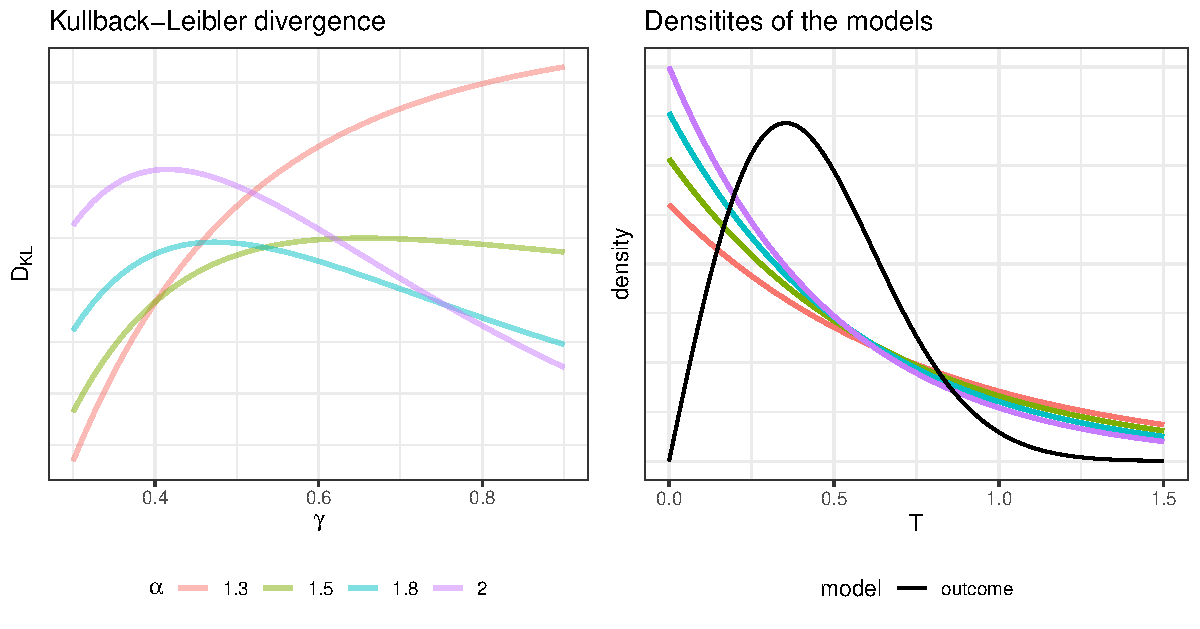
\includegraphics[width=.9\linewidth]{fig-mix-const-v1.pdf}
\end{center}
\end{onlyenv}

\begin{onlyenv}<2>
\begin{center}
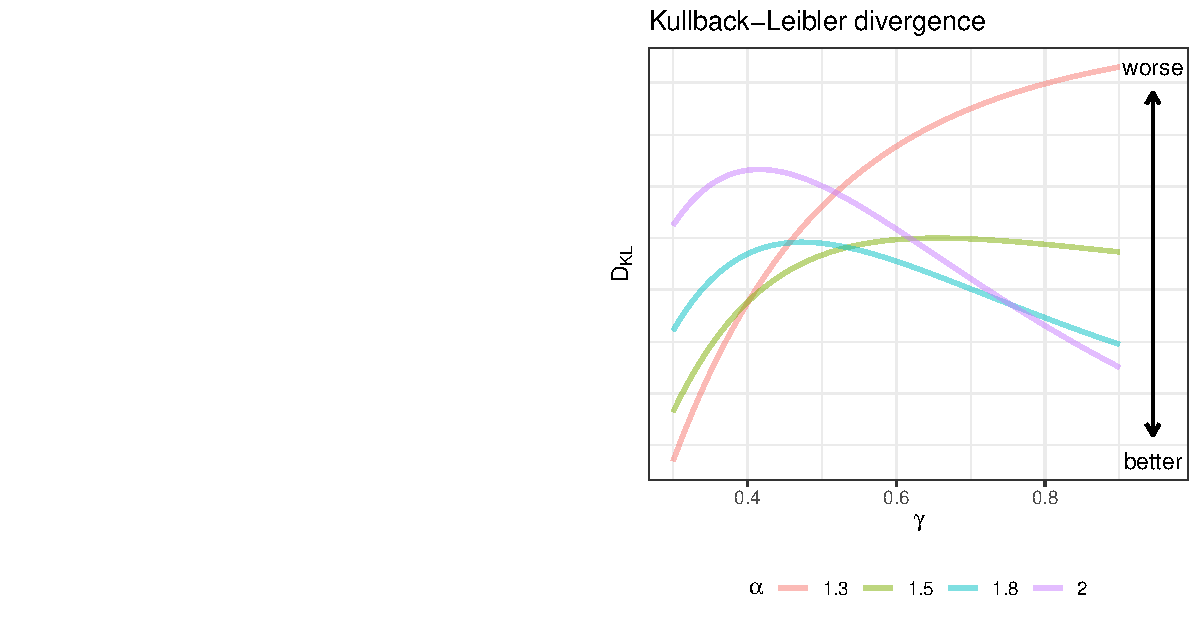
\includegraphics[width=.9\linewidth]{fig-mix-const-v3.pdf}
\end{center}
\end{onlyenv}

\begin{onlyenv}<3>
\begin{center}
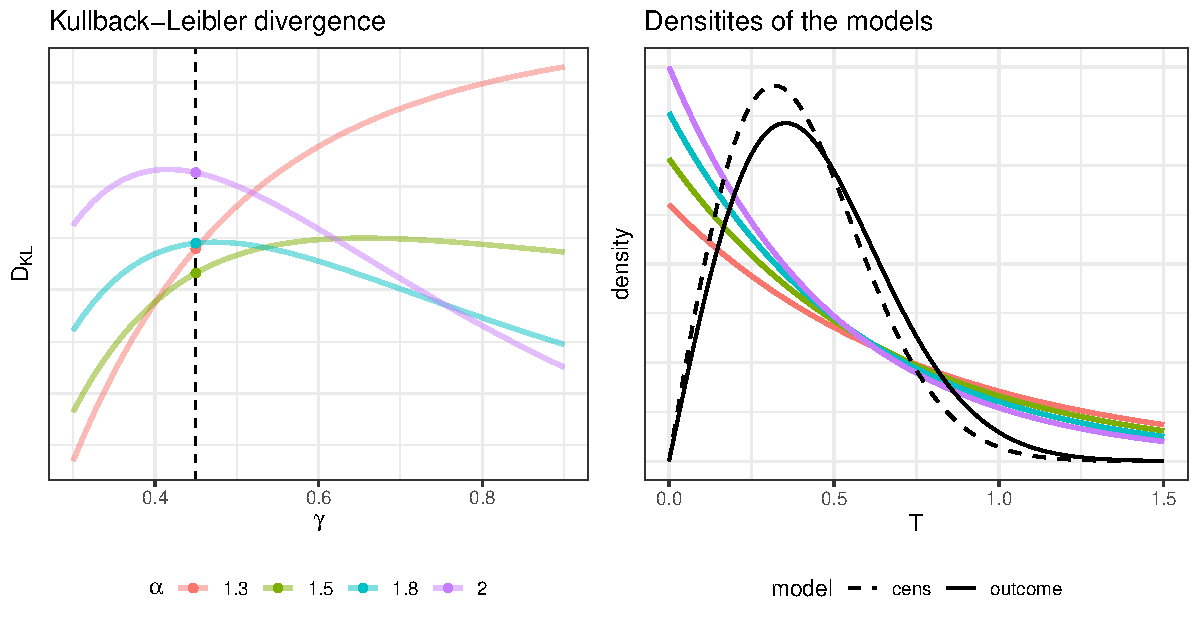
\includegraphics[width=.9\linewidth]{fig-mix-const-v2.pdf}
\end{center}
\end{onlyenv}
\end{frame}

\section{Hold-out samples and survival model estimators}
\label{sec:orgabd8c50}

\begin{frame}[label={sec:orgf346bc9}]{}
\begin{block}{\center Breaker}
\end{block}
\end{frame}


\begin{frame}[label={sec:org623d904}]{Survival curve estimators evaluated on hold-out samples}
[sort of: ignores this and proceeding anyway\ldots{}]
\end{frame}
\begin{frame}[label={sec:orgfb49f9a}]{Modeling the censoring}
\end{frame}
\begin{frame}[label={sec:org0054009}]{An (infinite?) loop}
\end{frame}

\section*{References}
\label{sec:org8ef4ed5}
\begin{frame}[label={sec:orga0f07ec}]{References}
\footnotesize \bibliography{./latex-settings/default-bib.bib}
\end{frame}
\end{document}